\documentclass{article}
\usepackage{graphicx} % Required for inserting images
\usepackage{geometry}
\usepackage{circuitikz}
\usepackage{siunitx}
\usepackage{CJKutf8}
\usepackage{amsmath}
\usepackage{amssymb}
\usepackage{caption}
\usepackage{float}
\usepackage{subcaption}
\geometry{top=5mm, left=30mm, a4paper}

\title{Feedback Circuit Prelab}
\author{梁程捷 (B11901136), 吳奕娃 (B11901080)}
\date{}


\begin{document}
\begin{CJK*}{UTF8}{bkai}

\maketitle

\section*{Feedback Circuit Active Filter}
\textbf{With input frequency range from 500 \unit{\hertz} to 200 \unit{\kilo\hertz}:}    \\
1. Find the maximum voltage gain $A_{max}$.   \\
2. Plot the band-pass amplitude-frequency curve.    \\
3. find $f_{L3dB\_BP}$, $f_{H3dB\_BP}$ and BW.    \vspace{3mm} \\ 
\textbf{Answer the following questions:}     \\
1. Is $f_{L3dB\_BP}$ equal to $f_{L3dB\_HP}$? If not, briefly describe it.    \\
2. Is $f_{H3dB\_BP}$ equal to $f_{H3dB\_LP}$? If not, briefly describe it.    \\


\begin{figure}[h]
    \begin{center}
    
        \begin{subfigure}[b]{0.8\textwidth}
            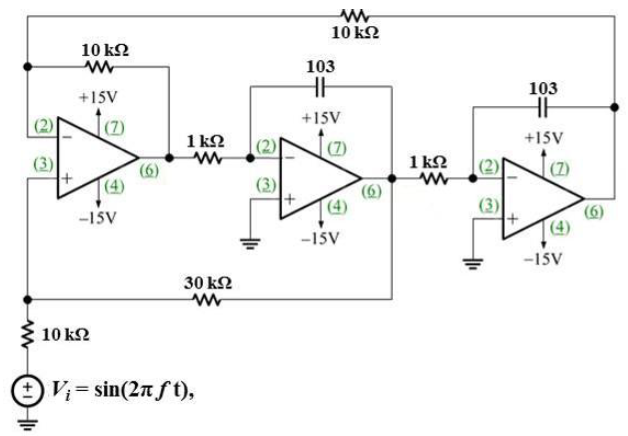
\includegraphics[width=\textwidth]{feedback_circuit.png}
            \caption*{\textbf{The feedback circuit}}
        \end{subfigure}
    \end{center}
\end{figure}

    
\end{CJK*}
\end{document}